\documentclass[12pt]{article}

\usepackage[margin=1in]{geometry}
%\usepackage{times}
\usepackage{mathptmx}
\usepackage{setspace}
\usepackage{lineno}
\usepackage{capt-of}
\usepackage{subcaption}
\usepackage{enumitem}
\usepackage[normalem]{ulem}
\usepackage{verbatim}

% section labels
\usepackage[small,compact,explicit]{titlesec}

%[numbers,sort&compress]
%removed to get full size citations as per their request
\usepackage{natbib}


\usepackage{graphicx}
\graphicspath{{images/}} 

\usepackage{url}
\urlstyle{same}

\renewcommand{\ULthickness}{0.75pt}

\titleformat{\section} {\vspace{6pt}\large\bfseries}{\thesection} {12pt} {#1\vspace{-6pt}}
\titleformat{\subsection} {\bf}{\thesubsection} {0pt} {#1\vspace{-12pt}}
\titleformat{\subsubsection}[runin]{\vspace{0pt}\normalfont\normalsize\bfseries}{\thesubsubsection} {6pt} {#1}

\usepackage{color,soul}
\sethlcolor{yellow}
\newcommand{\todo}[2]{\hl{\textbf{#1:} #2}}
\usepackage{booktabs}

\parindent 0pt
\parskip 12pt


\makeatletter
\newenvironment{figurehere}
{\def\@captype{figure}}
{}
\makeatletter

\setcitestyle{aysep={}}

\usepackage{xr}
\makeatletter
\newcommand*{\addFileDependency}[1]{% argument=file name and extension
  \typeout{(#1)}
  \@addtofilelist{#1}
  \IfFileExists{#1}{}{\typeout{No file #1.}}
}
\makeatother
 
\newcommand*{\myexternaldocument}[1]{%
    \externaldocument{#1}%
    \addFileDependency{#1.tex}%
    \addFileDependency{#1.aux}%
}
\myexternaldocument{main}


\onehalfspacing
\pagewiselinenumbers

\begin{document}



\begin{flushleft}

\baselineskip 24pt

{\Large Phylogenetic measures of indel rate variation among the HIV-1 group M subtypes: Supplementary Material}  % tentative

\end{flushleft}


\section * {Supplementary Figures}
%\todo{Art}{can't merge this title onto the next page with the GLM table}

\setcounter{table}{0}
\renewcommand\thetable{S\arabic{table}} 


\setcounter{figure}{0}
\renewcommand\thefigure{S\arabic{figure}} 


\begin{figure}[htbp]
    \centering
    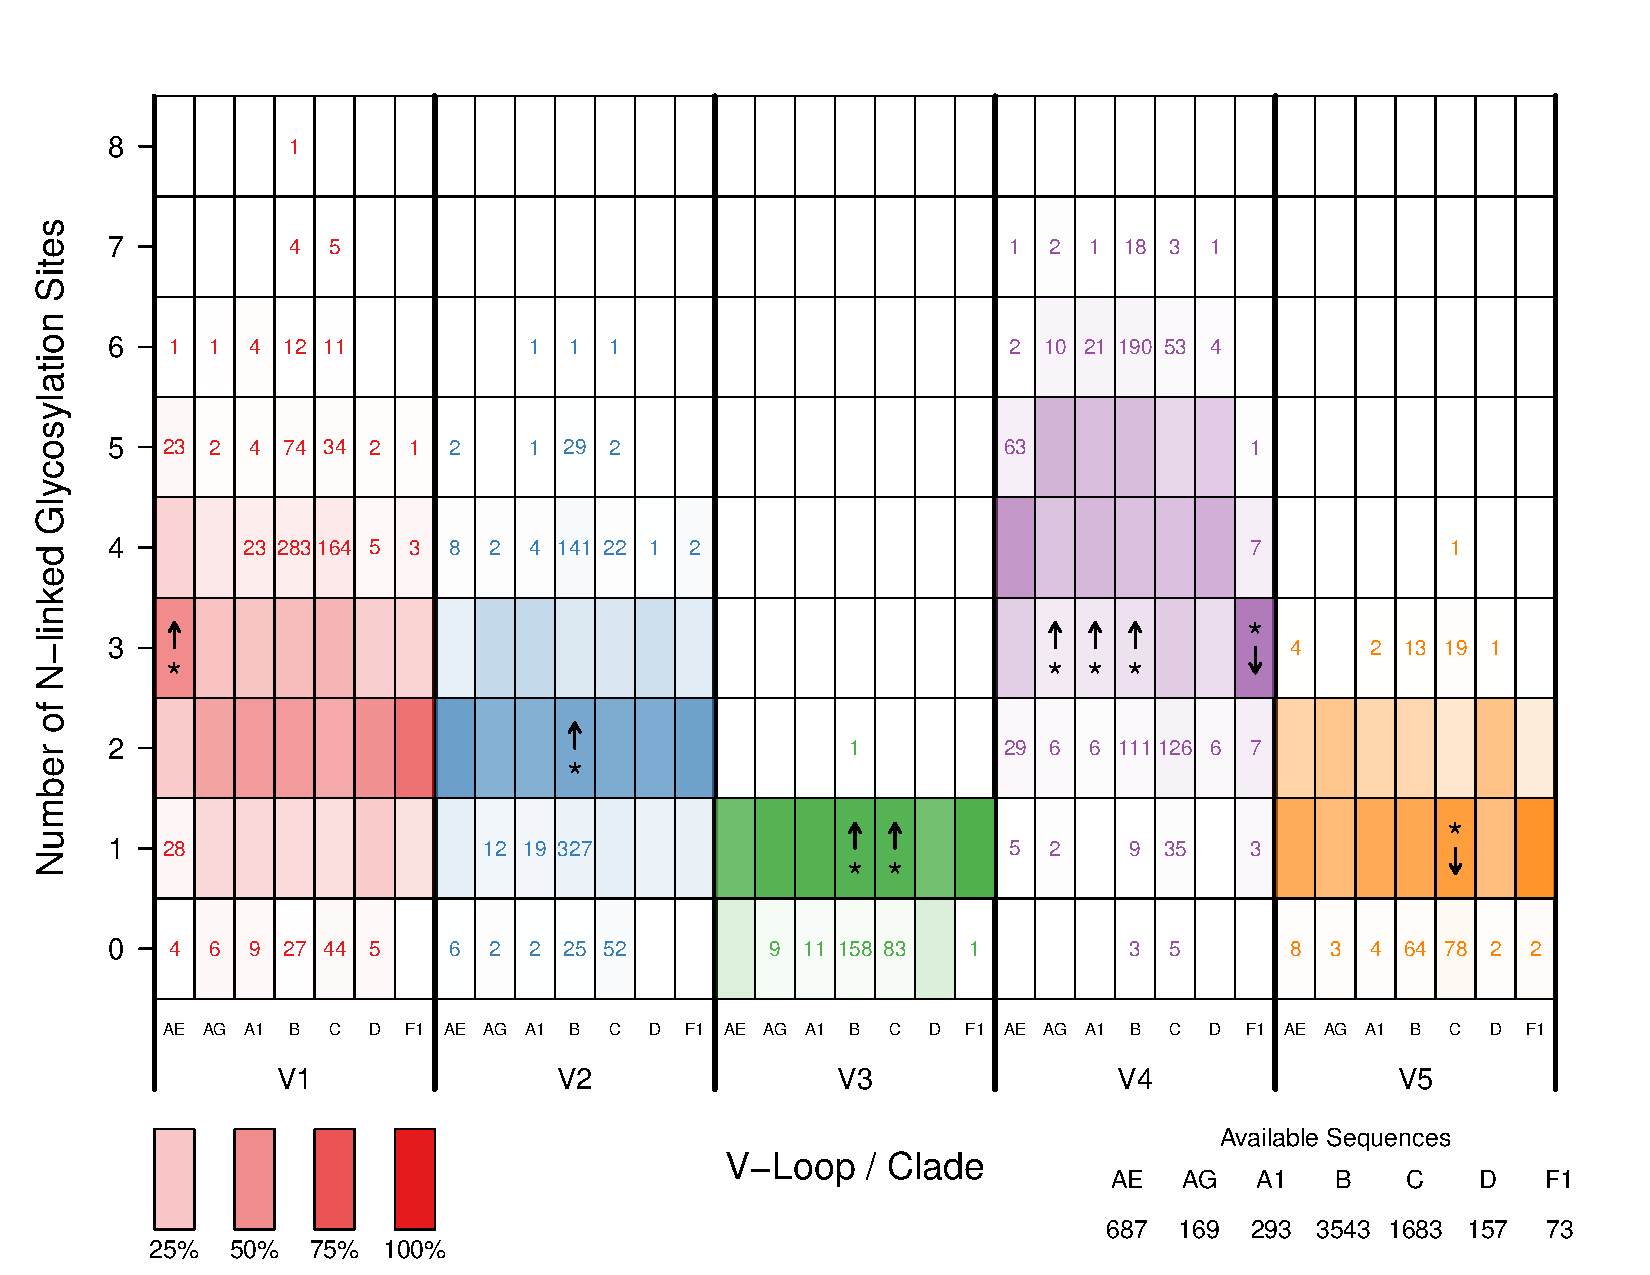
\includegraphics[width=.95\textwidth, trim={5mm, 0mm, 12mm, 15mm}, clip]{pngs-totals}
    \caption{The number of N-linked glycosylation sites in the variable loops of gp120.	
    Columns within each variable loop section describe the counts retrieved for one specific group M clade. 
    The color density of each box indicates the proportion of sequences containing the given count. 
    Examples of color densities and their corresponding proportions are provided by the four boxes to the bottom left of the figure.  
	Boxes containing a number highlight PNGS counts that are above zero, but contained less than 10\% of the distribution and therefore, did not generate a noticeable color.
    Asterisks (*) and arrows denote the presence and direction of significantly different PNGS counts among clades within a given variable loop (Poisson GLM).
    }
    \label{pngs-totals}
\end{figure}

\clearpage

\section * {Supplementary Tables}

\begin{table}[htbp]
\renewcommand{\arraystretch}{1.15}
  \centering
  \begin{tabular}{lrrcclrrc}
    \hline
   & Estimate & $P$ & Signif.   &&  & Estimate & $P$ & Signif. \\ 
    \cline{1-4} \cline{6-9}
    
    Time & 0.001 & $<10^{-15}$ & * & & Interactions \\ 
	Clade  &  &  &  &  & \hspace{1em}F1:V2 & -0.860 & 0.285 &  \\ 
  \hspace{1em}AE &  (reference) &  &  && \hspace{1em}AG:V3 & -2.073 & 0.063 &  \\ 
  \hspace{1em}AG & 1.946 & 0.058 &  &  &\hspace{1em}A1:V3 & 0.127 & 0.799 &  \\ 
  \hspace{1em}A1 & -0.103 & 0.741 &  & &\hspace{1em}B:V3 & -0.381 & 0.255 &  \\ 
  \hspace{1em}B & -1.156 & $1.6\times 10^{-10}$ & * & &\hspace{1em}C:V3 & -0.109 & 0.752 & \\ 
  \hspace{1em}C & -0.372 & 0.065 & &&\hspace{1em}D:V3 & 1.363 & 0.017 &  \\ 
  \hspace{1em}D & -0.639 & 0.070 & &&\hspace{1em}F1:V3 & -13.565 & 0.926 & \\ 
  \hspace{1em}F1 & -0.158 & 0.780 && & \hspace{1em}AG:V4 & -2.441 & 0.027 & \\ 
  Variable Region  & & & & &\hspace{1em}A1:V4 & -0.099 & 0.819 & \\ 
  \hspace{1em}V1 & (reference) & & & &\hspace{1em}B:V4 & -0.208 & 0.396 & \\
  \hspace{1em}V2 & -0.578 & 0.012 &  & &\hspace{1em}C:V4 & -0.215 & 0.428 & \\ 
  \hspace{1em}V3 & -4.448 & $<10^{-15}$ & * &  &\hspace{1em}D:V4 & 0.718 & 0.164 &\\ 
  \hspace{1em}V4 & -0.438 & 0.044 & & &\hspace{1em}F1:V4 & -0.577 & 0.439 &  \\ 
  \hspace{1em}V5 & -0.042 & 0.844 & & &\hspace{1em}AG:V5 & -2.455 & 0.022 & \\ 
  Interactions & & & &&\hspace{1em}A1:V5 & -0.569 & 0.151 & \\ 
  \hspace{1em}AG:V2 & -2.349 & 0.039 & & &\hspace{1em}B:V5 & 0.194 & 0.407 & \\ 
  \hspace{1em}A1:V2 & -0.457 & 0.313 &  &&\hspace{1em}C:V5 & 0.246 & 0.345 & \\ 
  \hspace{1em}B:V2 & -0.918 & $4.1\times 10^{-4}$& * & &\hspace{1em}D:V5 & -0.156 & 0.740 & \\ 
  \hspace{1em}C:V2 & -1.115 & $1.1\times 10^{-4}$ & * & &\hspace{1em}F1:V5 & -0.188 & 0.797 & \\ 
  \hspace{1em}D:V2 & -0.326 & 0.527 &  & &\\  
  
  \hline
  \end{tabular}
  
  \caption{
    Statistical comparisons generated by applying a generalized linear model to cherry indel analysis. 
    Comparisons made between clades and between variable regions were in relation to a reference group (AE and V1, respectively). 
    Effects of clade and variable region interactions were compared to predicted mean values to detect significant differences. 
    Groups with * symbols denoted statistically significant differences based on a Bonferroni-corrected threshold suited for multiple comparisons ($\alpha$ = 0.05/n). 
    }
    \label{tab:glm}
\end{table}

\end{document}
